This module deals with creation and interaction with the database.

\subsubsection{Use-cases}
After a project has been created a database collection is created and accociated with it, then the project can request and update the database and persist as shuffle criteria grows.\par
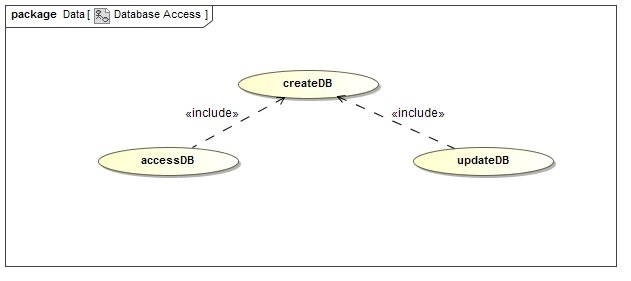
\includegraphics[width=13cm]{./graphics/databaseAccessUseCase.jpg}
    \rule{0\linewidth}{0.15\linewidth}\par
\begin{enumerate}
\item createDB\par
Priority: Critical.\par


\end{figure}
\item accessDB\par
Priority: Critical.\par

\item updateDB\par
Priority: Critical.\par


\end{enumerate}